\chapter{État de l'art}

	Ce chapitre a pour intention de définir et préciser les différentes notions nécessaires à la lecture des travaux de thèses, ainsi que de définir le contexte scientifique du travail. Il portera, dans une première section, sur les détails des différents transferts de flot d'exécution dans les systèmes modernes, ainsi que les changements d'états inhérents à ces transferts de flot d'exécution. Cette section abordera ensuite les problèmes de sécurité liés au transfert de flot d'exécution, ainsi que les techniques de mitigation de ces problèmes. Cette section terminera sur les problématiques temps réel touchant au transfert de flot d'exécution.
	La seconde section de ce chapitre fera un état des lieux de la preuve de programme. Elle commencera par discuter de ce qu'est une preuve et de leur vérificaton automatique, ainsi que des stratégies de conduite de preuve. Cette section continuera sur la preuve de programme, en particulier comment raisonner sur un programme impératif. Elle abordera aussi les notions de représentation du langage. Enfin, elle terminera sur les exemples de systèmes vérifiés formellement.

	\section{Transfert de flôt d'exécution}
	\label{control_flow_transfer}

		\subsection{Définitions}

		\paragraph{Flôt d'exécution}

\label{context}
			Un flôt d'exécution est une trame de modifications successives de l'état de la machine, animée par la récupération et l'exécution machinale d'instructions assembleur contigües par le processeur. Cette trame est l'oeuvre d'une entité qui a conçu le code et les conditions d'exécution permettant d'aboutir à un résultat. Ces conditions d'exécution (ou \emph{contexte d'exécution}) peuvent comprendre n'importe quel sous-ensemble de l'état de la machine, comme l'état de certains registres du processeur ou l'état d'une partie la mémoire par exemple. Une certaine notion de confiance est liée à chaque fil d'exécution, qui peut se refléter sur les droits accordés à celui-ci.

		\paragraph{Transfert de flôt d'exécution}

			Le transfert de flôt d'exécution est le fait de faire diverger un flôt d'exécution vers un autre. Il existe de nombreuses utilisations du transfert de flôt d'exécution, mais nous en distinguerons deux types : les transferts de flôt d'exécutions internes et les transferts de flôt d'exécution externes.

			Seront considérés comme des transferts de flôt d'exécution \emph{internes} les transferts de flôt d'exécution qui ciblent un fil d'exécution conçu par la même entité que le fil d'exécution  initial. Les deux fils d'exécutions sont conçus pour coopérer et ce type de transfert de flôt d'exécution se déroule typiquement sans changement de droits. Un premier exemple d'un tel transfert de flôt d'exécution, le plus simple, est le saut : il permet de définir de manière arbitraire l'adresse de la prochaine instruction à exécuter. Similairement, le saut conditionnel permet d'effectuer un saut en fonction du résultat d'une instruction assembleur, divisant le flot d'exécution en deux fils possibles. Les appels de fonctions sont un exemple plus complexe de transferts internes ; contrairement aux sauts, les appels de fonctions permettent de revenir au flôt d'exécution initial. Dès lors, à chaque appel de fonction, il est nécessaire de sauvegarder la portion de l'état qui sera modifiée par effet de bord lors de l'exécution de la fonction.  La portion de l'état modifié par la fonction est connue par l'entité, qui peut donc réaliser une sauvegarde partielle minimale de l'état sans perte d'information sur l'état.

			Les transferts de flôt d'exécution \emph{externes} sont ceux qui -- par opposition aux transferts de flôt d'exécution internes -- impliquent un transfert de flôt d'exécution vers le fil d'exécution d'une autre entité. Ce type de transfert peut se traduire par un changement de droits liés au fil d'exécution, reflétant les droits de la nouvelle entité. Les transferts externes peuvent aussi engendrer une sauvegarde du contexte d'exécution initial ; cependant, à l'instar des transferts internes, il n'est pas possible de savoir quelles portions de l'état sont susceptibles d'être modifiées par l'autre entité. Ainsi, un tel transfert implique une sauvegarde préventive complète du contexte d'exécution susceptible d'être modifié par l'autre entité.

\textcolor{red}{J'ai envie de parler de la limite des contextes d'exécution, notamment avec les attaques micro architecturales mais je n'arrive pas à le formuler} Il est difficile de déterminer ce qui fait partie de l'état d'un programme : le contenu des registres du processeur et de la mémoire, mais aussi l'état des composants logiciels ou matériels intéragissant avec le programme (tels que les périphériques, le cache, etc.).

			De plus, chaque fil d'exécution ciblable par un transfert externe doit être muni d'un cadre d'exécution, qui spécifiant le point d'entrée, l'environnement initial, et les droits liés à ce fil d'exécution. Ils servent à s'assurer que le flôt d'exécution ne sera exécuté que dans les conditions prévues par l'entité qui l'a conçu. Cela implique que l'intégrité des cadres d'exécution de chaque entité doit être garanti au sein d'un système ; une entité ne doit pas pouvoir altérer les cadres d'exécution d'une autre entité.

			Ce document discutera principalement des transferts de flôt d'exécution externes. La prochaine sous-section présentera des exemples de transferts de flôt d'exécution externes au sein d'un système. 

		\subsection{Transferts de flôt d'exécution externes au sein d'un système}

			\subsubsection{Appels explicites}
			Les transferts externes les plus courants sont les transferts de flot d'exécution explicites, c'est-à-dire dont la cible est explicitement fournie lors de l’appel, ou clairement établie dans la documentation.

Par exemple, dans Linux, un processus peut demander l’ouverture d’un fichier avec l’appel système \texttt{open()}. Cet appel transfère le flot d’exécution d’un processus non privilégié vers le noyau Linux disposant du plus haut niveau de privilèges. Les fonctions appelables par des transferts explicites servent d’interface entre des logiciels disposant de droits distincts. Dans le cas de Linux, le cadre d'exécution a été défini par Linux, qui prend les dispositions de sauvegardes nécessaires afin de pouvoir rétablir le contexte d'exécution du processus appelant au moment du retour de l'appel système.

			\subsubsection{Fautes}
\label{sec:faults}
Les différentes formes de fautes logicielles constituent aussi une forme de transfert de flot d'exécution externes. Les logiciels sont susceptibles de déclencher des fautes logicielles de différentes façons, par exemple :
\begin{itemize}
  \item décodage impossible de la prochaine instruction ;
  \item demande d'exécution d'une instruction impossible (division par zéro...) ; 
  \item demande d'accès à une adresse mémoire protégée, résultat de l'activité d'une MMU ou d'un autre dispositif matériel (MPU, Trustzone, SGX) ;  
  \item demande d'exécution d'une instruction privilégiée en mode non-privilégié.
\end{itemize}
Dans ces différentes situations, il s'agit de transferts implicites depuis le logiciel en faute vers une fonction d'un logiciel en charge du traitement de cette faute. Les différentes fonctions de gestion des fautes sont généralement définies par des éléments de configuration du matériel, et, le plus souvent, par l'intermédiaire d'une table (ou vecteur) dont le nom change d'une architecture de microprocesseur à l'autre. Ce vecteur précise généralement le niveau d'élévation de privilèges associé à l'exécution de la fonction de traitement de la faute. Cette table précise en réalité le cadre d'exécution des fils d'exécutions dédiés à chaque fautes. Sur les architectures Intel cette table est appelée \emph{IDT} (pour \emph{Interrupt Descriptor Table}).
\label{IDT}

			\subsubsection{Interruptions matérielles}
			Les interruptions matérielles sont des transferts non explicites \textit{a priori} non contrôlés par le code non privilégié. Elles sont déclenchées par le matériel, signalant un événement important à traiter, tel que l'arrivée d'un paquet réseau par exemple. Les fonctions de traitement des interruptions matérielles ainsi que leur cadre d'exécution sont aussi définis dans l'\emph{IDT} dans l'architecture Intel x86.

		\subsection{Implications logicielles d'un transfert de flot d'exécution}

			\subsubsection{Changement de droits}

Sur l'architecture Intel x86, les différents transferts de flot d'exécution peuvent s'opérer par le biais de différentes instructions et événements matériels. Néanmoins, lorsqu'un changement de droits est requis lors d'un transfert, les différents chemins sont régis par un ensemble de mécanismes de contrôle relativement homogènes.

\paragraph{Changement de droits sous x86}
\label{ring}

Les privilèges attribués au code s'exécutant actuellement sur la machine sont ceux du \emph{segment} chargé dans le registre \texttt{CS} (pour \emph{code segment}). Les segments sont définis dans la \emph{GDT} (pour \emph{Global Descriptor Table}) à l'initialisation de la machine. La \emph{GDT} est une table globale spécifiée par Intel, dont l'adresse est accessible par un registre dédié. Dans cette table par exemple, Linux se contente de définir deux segments de code. Un premier segment associé au niveau de privilèges maximum du microprocesseur, nommé par Intel \emph{ring 0}, utilisé pour le code responsable du système ; et un second segment non-privilégié, associé au niveau de privilèges \emph{ring 3}, pour le reste du code. 

Contrairement au code s'exécutant avec le segment privilégié, le code s'exécutant sans privilège ne peut pas changer de segment à sa guise. Des mécanismes de contrôle du processeur déclenchent une faute si du code non-privilégié essaie de modifier son segment de code. Pour y parvenir, il est possible d'utiliser les \emph{gates}, qui sont des tremplins définis dans les tables globales du système (comme l'\emph{IDT} ou la \emph{GDT}), permettant au code non privilégié d'appeler une fonction prédéfinie qui s'exécute avec d'autres droits.

Lorsqu'un changement de segment déclenche un changement de niveau de privilèges, le processeur change de pile. Ce changement de pile permet d'éviter aux routines privilégiées les échecs dus à un manque de place sur la pile, ainsi qu'à les prémunir d'éventuelles interférences avec les procédures non privilégiées~\cite{intel_stack_switch}. 
Une pile doit être définie par niveau de privilèges (\emph{ring}) utilisé par le système ; leurs adresses doivent être renseignées dans une structure appelée \emph{TSS} (pour \emph{Task State Segment}). Cette structure est initialisée conjointement avec la \emph{GDT} qui contient son descripteur. Un registre dédié indique au processeur la position de ce descripteur dans la \emph{GDT}.

\paragraph{Appels systèmes sur x86}

Afin d'obtenir un transfert de flot d'exécution avec élévation de privilèges, le logiciel appelant non-privilégié peut exécuter des instructions dédiés aux différentes \emph{gates} des tables globales. Tout d'abord, l'instruction \texttt{int} permet d'appeler les \emph{gates} situées dans l'\emph{IDT}. Ces \emph{gates} sont soit des \emph{interrupt gates}, des \emph{trap gates} ou des \emph{task gates}~\cite{intel_idt_gates}. \texttt{int} s'accompagne d'un argument correspondant à l'index de la \emph{gate} ciblée dans l'\emph{IDT}. Le code ainsi appelé sera exécuté avec le niveau de privilèges spécifié par le segment de code indiqué dans la gate (et chargé dans le registre \texttt{CS}).

\label{sec:x86_syscall}
D'autres instructions telles que \texttt{lcall} ou \texttt{ljmp} permettent d'utiliser les \emph{gates} situées dans la \emph{GDT}. Ces gates sont soit des \emph{call gates} ou des \emph{task gates}. Ces gates permettent de copier un nombre fixé d'arguments depuis la pile de l'appelant dans la pile du code privilégié à l'appel de ces instructions. Le nombre d'arguments à copier est renseigné dans la \emph{gate} ciblée par l'instruction. Là aussi, l'élevation de privilèges est spécifiée par le segment de code indiqué dans la gate et chargé dans \texttt{CS} lors de l'appel.

La troisième manière de déclencher une élévation de privilèges est l'instruction \texttt{sysenter}. Cette 
instruction ne sollicite aucune \emph{gate} : à la place, elle utilise les \emph{MSR} (pour \emph{model-specific registers}), qui sont des registres de contrôle du processeur. Ces \emph{MSR} sont manipulables grâce aux instructions \texttt{wrmsr} et \texttt{rdmsr}, qui sont des instructions privilégiées et qui permettent d'écrire et de lire dans ces registres respectivement. Un appel à \texttt{sysenter} utilise les MSR \texttt{0x174}, \texttt{0x175} et \texttt{0x176} pour charger \texttt{CS} \texttt{EIP} \texttt{SS} \texttt{ESP}. Le système doit donc avoir initialisé ces registres avant l'utilisation de \texttt{sysenter}. De plus, \texttt{sysenter} ne sauvegarde pas l'adresse de retour ni l'adresse de la pile lors d'un appel, qui doivent être placés dans les registres \texttt{ECX} et \texttt{EDX} au moment de l'appel à \texttt{sysexit} pour retourner dans le code appelant.

\paragraph{Interruptions et fautes sur x86}

Les interruptions liées au matériel sur l'architecture x86 étaient autrefois gérées par un coprocesseur (le PIC 8259 \emph{pour Programmable Interrupt Controller} ou plus récemment, l'APIC pour \emph{Advanced Programmable Interrupt Controller}). Ce coprocesseur est maintenant intégré au processeur, mais nous continuerons de parler de coprocesseur pour honorer l'histoire. Ce coprocesseur utilise les \emph{gates} situées dans l'IDT de la même manière que l'instruction \texttt{int}. Il est possible de configurer ce coprocesseur
pour qu'il utilise une certaine plage de niveaux d'interruption, ou pour qu'il masque temporairement la venue de nouvelles interruptions. Les fautes utilisent elles aussi l'\emph{IDT}, et utilisent les trente-deux premières \emph{gates} de la table, en fonction de la faute à déclencher. Les fautes et interruptions déclenchées par le processeur ou le coprocesseur ont toujours le droit d'utiliser les \emph{gates}, peu importe le niveau de privilèges du code s'exécutant au moment de l'interruption.

\paragraph{Fonctionnement de la \emph{MMU} sur l'architecture Intel 32 bits}
\label{sec:intel_mmu}
Sur l'architecture Intel x86, mais aussi sur toutes les autres architectures supportant une \emph{MMU} (pour \emph{Memory Management Unit}), il est possible d'associer des droits d'accès spécifiques à chaque pages de mémoire configurée dans l'espace d'adressage virtuel.

Le concept de traduction d'adresse virtuelle vers l'adresse réelle est le suivant. Les bits de poids forts de l'adresse virtuelle servent à traverser les tables de la MMU (sur l'architecture Intel x86, le \emph{Page Directory} et les \emph{Page Tables}). Les bits de poids faible correspondent à l'emplacement de l'adresse désirée dans la page réelle obtenue après traduction (souvent appelé \emph{offset}).

En particulier, sur Intel x86 et en mode de pagination 32 bits pour des pages de 4 Kio, les espaces d'adressage sont configurés par une structure de données arborescente de pages de 4Kio. Cette structure de données a deux étages : la racine appelée PD pour \emph{Page Directory}, et les feuilles appelées PT (pour \emph{Page Tables}). Le développeur renseigne l'adresse du Page Directory à utiliser dans le registre \texttt{CR3} du processeur ; cette adresse est alignée sur 4Kio, les 12 bits de poids faibles (11-0) sont ignorés ou sont réservés pour un autre usage.

Plus précisement, le \emph{Page Directory} est constitué de 1024 entrées de 32 bits appelées les \emph{PDE} (pour \emph{Page Table Entries}). Les 20 bits de poids fort (31-12) de ces entrées déterminent l'adresse de la \emph{Page Table} à utiliser, alignée sur 4Kio. Les \emph{Page Tables} sont aussi constituée de 1024 entrées de 32 bits appelées \emph{PTE} (pour \emph{Page Table Entries}). De la même manière, les 20 bits de poids forts (31-12) déterminent l'adresse de la page de mémoire réelle, alignée sur 4Kio. (Il est aussi possible de configurer des pages de 4Mio plutot que des pages de 4Kio en modifiants certains bits de controle des \emph{PDE}.)

Lors de la traduction d'une adresse virtuelle, les 10 bits de poids forts de l'adresse virtuelle (31-22) déterminent le numéro de \emph{PDE} à utiliser, les bits (21-12) déterminent le numéro de \emph{PTE}, et les 12 bits de poids faible restants (11-0) déterminent l'\emph{offset} de l'adresse cible dans la page réelle.~\cite{intel_32bits_paging}

\paragraph{Contrôle d'accès par la MMU sur Intel x86}
Dans le mode de pagination 32 bits d'Intel, les droits associés à chaque page sont présents dans les \emph{PTE}, dans les 12 bits de poids faible. Le bit 1 (\texttt{R/W}) permet d'empêcher les accès en écriture sur la page. Le bit 2 (\texttt{U/S}) permet d'empêcher n'importe quel accès utilisateur à la page - en lecture ou en écriture. Le niveau de privilège de l'accès dépend du \emph{CPL} (pour \emph{Current Privilege Level}) de l'instruction courante, souvent déterminée par le segment de code actuel.
L'architecture Intel permet de restreindre la récupération des instructions en discriminant chaque page de mémoire. Cette fonctionnalité n'est cependant pas disponible dans le mode de pagination 32 bits, puisqu'elle nécessite des \emph{PDE} ou \emph{PTE} longues de 64 bits. Elle est par exemple disponible dans le mode de pagination \emph{PAE}. Cette fonctionnalité est activable au travers du bit \texttt{NXE} du registre \texttt{IA32\_EFER}. Pour chaque page de mémoire, mettre le bit 63 (\texttt{XD}) à 1 dans une \emph{PTE} empêche la récupération d'instruction depuis cette page mémoire.

Cependant, d'autres fonctionnalités de contrôle d'accès globaux liées à la \emph{MMU} existent. L'architecture Intel propose aussi les mécanismes \emph{SMAP} et \emph{SMEP} comme décris dans le paragraphe \ref{memory_rights}.
Le bit \emph{SMAP} (pour \emph{Supervisor Mode Access Protection} présent dans le registre CR4 permet d'empêcher du code utilisant un segment de données privilégié d'accéder aux pages mémoire annoncées comme étant des pages mémoire utilisateur (bit \texttt{U/S} à 1).
Le bit \emph{SMEP} pour \emph{Supervisor Mode Execution Protection} présent dans le registre CR4 permet d'empecher la récupération de code lorsque le segment actuel octroie des accès privilégiés et que la page mémoire contenant les instructions est annoncée comme une page mémoire utilisateur (bit \texttt{U/S} à 1).

			\subsubsection{Capture de l'état d'exécution}


%Le contexte d'exécution d'un programme est constitué d'informations permettant de reprendre de manière saine l'exécution d'un programme à un moment arbitraire de son exécution après qu'il ait été interrompu. Le contexte d'exécution est donc intimement lié à l'état de la machine lors de l'exécution du programme. 

%Le contexte d'exécution d'un programme doit contenir toute partie de l'état du programme susceptible d'être modifiée légitimement par d'autres programmes du système. De ce fait, il n'est pas nécessaire de copier la mémoire utilisée par le programme. Dans les systèmes d'exploitation modernes, chaque programme dispose d'une portion de mémoire qui lui est dédiée. Cela peut être garanti par conception dans le cas de systèmes collaboratif ou plus strictement par des mécanismes de controle d'accès relatifs à une \emph{MMU} ou une \emph{MPU} par exemple. 
%Puisqu'il n'est pas nécessaire de copier le contenu de la mémoire, il suffit donc de copier les registres du processeur susceptibles d'être modifiés. Lors d'appels sans changement de droit, des règles de sauvegarde des registres existent (par exemple \cite{arm32_bit_callconv}). Ces règles décrivent notamment quels sont les registres susceptibles d'être modifiés par l'appelé, et peuvent permettre d'économiser la sauvegarde de certain registres.
%%Cependant, puisque les transferts de flot d'exécution avec changement d'espace d'adressage et de droits peuvent être implicites, le système ne peut faire aucune hypothèse sur les registres préalablement sauvegardés par le programme interrompu. De plus, il est courant de continuer l'exécution d'un autre programme susceptible de modifier n'importe quel registre à sa disposition. En toute généricité, il est donc impossible de prévoir quels registres resteront intacts lors d'un tel transfert : il est donc nécessaire de sauvegarder tous les registres modifiables par le programme interrompu.
Lorsqu'un transfert de flôt d'exécution externe survient, un changement de contexte d'exécution doit être effectué, assisté par le processeur. En effet, sans l'aide du processeur, le contenu de certains registres comme le pointeur d'instruction ou le pointeur de pile seraient instantanément perdus au moment du transfert. Voici comment se passe le transfert pour chaque mode de transfert différent sous l'architecture Intel x86 : 


\paragraph{Changement de pile et registres sauvés lors d'un appel au travers d'une \emph{callgate}}
\label{sec:intel_callgate}

Lors d'un tel appel, le processeur accède à la \emph{callgate} par la \emph{GDT}. Cette callgate indique entre autres, le segment de code à utiliser (et donc le niveau de privilège associé), l'emplacement du code à exécuter, le nombre d'arguments à copier depuis la pile utilisateur. La pile ainsi que le segment à utiliser sont eux renseignés dans la \emph{TSS} et sont liés au niveau de privilège du segment de code de la callgate.

Tout d'abord, le processeur sauve de manière temporaire le segment de pile et le pointeur de pile dans un tampon interne. Il remplace les registres de segment de pile et de pointeur de pile par ceux renseignés dans la \emph{TSS}, changeant de pile. Il pousse ensuite le segment de pile et le pointeur de pile de l'utilisateur dans la nouvelle pile. Il copie ensuite les arguments depuis la pile utilisateur vers la nouvelle pile, leur nombre étant renseigné dans la call gate. Le processeur pousse ensuite sur la pile le registre de segment de code et le pointeur d'instruction, avant de les remplacer par ceux renseignés dans la call gate.

\paragraph{Changement de pile et registres sauvés lors d'une interruption, d'une faute ou d'un appel à \texttt{int}}
\label{intel_hard_context}
Lors d'une faute, d'une interruption ou d'un appel à \texttt{int}, le processeur accède à une interrupt gate ou une trap gate dans l'\emph{IDT}. Comme pour la call gate, la gate contient le segment de code à utiliser, le code à exécuter. Ce transfert de flot d'exécution n'entraine pas une copie par le processeur d'éventuels arguments depuis la pile utilisateur sur la nouvelle pile.

Tout d'abord, le processeur change de pile, en sauvant temporairement les valeurs utilisateurs du segment de pile \texttt{SS} et de la pile \texttt{ESP}, et en les écrivants sur la pile renseignée dans la nouvelle pile renseignée dans la \emph{TSS}. Le processeur sauve ensuite l'état des registres \texttt{EFLAGS}, du segment de code \texttt{CS} et du pointeur d'instruction \texttt{EIP}. EFLAGS contient entre autres l'état des drapeaux d'overflow, de retenue, de parité, de conditions, mais aussi d'activation des interruptions. Le processeur peut pousser un code d'erreur supplémentaire sur la pile dans le cas de déclenchement de certaines fautes afin de préciser leur cause.

		\subsection{Sécurité liée aux transferts de flôt d'exécution}

		Les transferts de flôt d'exécution (internes ou externes) sont un des points clés de la sécurité d'un système. Pour prendre le contrôle d'un système, une entité pourrait essayer de corrompre les transferts de flôt d'exécution se tenant à l'intérieur du système pour réussir à exécuter son propre fil d'exécution dans le système.

		Ainsi, ce document distinguera deux catégories majeures d'attaques : les attaques visant les transferts de flôt d'exécution internes, et les attaques visant les transferts de flôt d'exécution externes.

		\subsubsection{Sécurité relative aux transferts de flôt d'exécutions internes}
Ce type de transfert de flôt d'exécution, d'apparence assez anodine, est pourtant l'objet d'attaques multiples, dont le but est de faire dévier l'exécution (de préférence en mode privilégié) vers du code choisi par l'attaquant. Pour y arriver, un attaquant doit exploiter une vulnérabilité dans une portion de code, qui lui donnera le contrôle d'une zone de mémoire d'intérêt (la pile, le tas, ou même le code). Une fois qu'il contrôle cette zone mémoire, il lui suffit d'écrire un \emph{shellcode}, et d'exploiter une vulnérabilité dans du code privilégié pour que l'exécution du \texttt{return} de la fonction compromise saute dans le shellcode. L'attaquant gagne à ce moment le contrôle de la machine.

Commence alors un jeu du chat et de la souris pour essayer de mitiger l'impact de ces vulnérabilités. Pour compliquer la vie de l'attaquant, et qu'il lui soit plus difficile d'exécuter son shellcode, de nombreuses stratégies ont été entreprises par les fabriquant de matériels ainsi que par les développeurs de systèmes d'exploitation. 

\paragraph{Canaries}
Une première statégie est l'ajout de \emph{canary} qui visent à détecter les corruptions mémoires. Les canaries sont des valeurs écrites dans la pile ou le tas et qui sont générées aléatoirement à chaque exécution. Lors de la sortie de la frame protégée par le canary, le code vérifie que la valeur du canary correspond bien à celle qui avait été écrite initialement ; si ce n'est pas le cas, c'est qu'une corruption mémoire a eu lieu et une faute est levée.

Une des techniques permettant de vaincre les canaries est de lire la valeur initiale du canary avant de corrompre la mémoire. En effet, la canary \textbf{reste la même pour l'intégralité de l'exécution}. Une fois cette valeur récupérée, il suffit de corrompre la mémoire en réécrivant cette valeur au bon endroit pour échapper à la détection. De plus, si l'exploitation de la vulnérabilité permet de corrompre la mémoire de manière fine, il suffit d'éviter d'écrire sur la canary.

\paragraph{Droits fins pour les zones mémoires}
\label{memory_rights}
Une autre stratégie a été de définir des droits fins concernant l'accès aux différentes zones mémoires de l'espace d'adressage des processus. Le mécanisme de mémoire virtuelle permet de définir des droits d'accès propres à chaque page mémoire configurée (lecture, écriture, éxecution, accessible en mode non privilégié). Par exemple, les pages mémoire contenant du code sont typiquement configurées pour des accès en lecture et exécution, alors que les pages contenant des données (pour la pile, le tas, les sections de données d'un binaire) sont configurées pour des accès en lecture/écriture.

Cette stratégie de défense empêche un attaquant d'exploiter une vulnérabilité pour écrire un shellcode code dans la mémoire si on considère que chaque page de mémoire est soit exécutable, soit accessible en écriture. Cependant, il existe des cas d'usage légitimes qui violent cette contrainte, par exemple lors de compilation à la volée (ou JIT, pour Just-In-Time). Fatalement, de tels logiciels sont devenus la cible privilégiée des attaquants, on pourra par exemple citer Webkit \cite{webkitexploit}.
Heureusement, il est peu probable que de tels logiciels aient besoin de s'exécuter en mode privilégié. 

Pour affaiblir ce vecteur d'attaque, cette stratégie de défense est renforcée par des mécanismes de sécurité supplémentaires tels que le \emph{Supervisor Mode Access Prevention} (SMAP) et le \emph{Supervisor Mode Execution Prevention} (SMEP). SMAP permet au processeur de lever une faute lorsque qu'il exécute du code privilégié et qu'il essaie d'accéder (en lecture ou en écriture) à des données présentes dans l'espace utilisateur. SMEP permet en complément de lever une faute lorsque le processeur essaie d'exécuter du code dans l'espace utilisateur alors qu'il se trouve dans un mode d'exécution privilégié.

Ces mécanismes permettent d'isoler le code privilégié de potentiels shellcodes écrit en espace utilisateur. Ainsi, pour compromettre intégralement un système, l'attaquant doit à présent exploiter une vulnérabilité dans le code privilégié, ayant à sa disposition des pages mémoire soit accessibles en écriture soit exécutables et qui, de surcrois, ne font pas partie de l'espace utilisateur.
Nait alors une nouvelle technique d'exploitation de vulnérabilité. 

\paragraph{Return Oriented Programming}
\label{ROP}
Le ROP (pour \emph{Return Oriented Programming}) consiste à attaquer du code vulnérable en n'utilisant que le code déjà accessible dans l'environnement d'origine, mais en exécutant des portions arbitraires de celui-ci. L'attaque consiste à repérer des \emph{gadgets} : de brèves portions de code ayant un effet spécifique sur la mémoire ou les registres, suivi d'une instruction \texttt{return}. Pour l'attaquant, il suffit de dévier le flot d'exécution sur l'un de ces gadgets et de manipuler la mémoire, de manière à ce que l'exécution du gadget entraine l'exécution du suivant. L'attaquant parvient au final à exécuter son shellcode constitué d'une succession de gadgets, contournant les mécanismes de sécurité mentionnés dans le paragraphe précédent.\\

Plusieurs contre-mesures ont émergé pour rendre plus difficile le ROP.

\paragraph{Address Space Layout Randomization}
\label{aslr}
L'ASLR (pour \emph{Address Space Layout Randomization}) rend imprédictible l'adresse des différentes zones de mémoire au sein d'un espace d'adressage virtuel. Les adresses du binaire, de la pile, du tas, des librairies, du noyau, etc. sont rendus aléatoires à chaque nouvelle exécution. L'ASLR est de ce fait un frein considérable au développement d'un shellcode en ROP, puisqu'il est impossible de prédire où se situeront les gadgets lors de la prochaine exécution.

L'ASLR n'est cependant pas parfait. Les adresses des zones mémoire restantes peuvent être révélées par des pointeurs dans les zones mémoires controlées par l'attaquant \cite{bypasskaslr}, ou grâce à des attaques micro-architecturales \cite{microarchitecturalbypass}.

\paragraph{Vérification de l'intégrité du flôt d'exécution}
\label{cfi}
Une autre approche permettant de réduire la marge de manoeuvre de l'attaquant et de vérifier que le flot d'exécution est conforme à celui attendu. À chaque appel et à chaque retour de fonction, le processeur vérifie si la cible du saut est valide. Plusieurs implémentations existent, notamment des implémentations matérielles au sein des processeurs \cite{intelpointerauth, armpointerauth}, mais aussi certaines implémentations logicielles notamment provenant de compilateurs \cite{compilerpointerauth}. Windows, macOS, Android, iOS utilisent déjà un mécanisme de vérification du flot d'exécution.

\paragraph{eXecute Only Memory}
\label{execute_only_memory}
Le XOM (pour \emph{eXecute Only Memory}), est une fonctionnalité de certain processeurs permettant de déclencher une faute lorsqu'un accès en lecture est fait sur les pages mémoires configurées comme étant exécutables. Avant cette fonctionnalité, aucune distinction n'était faite entre le processus de récupération des instructions par le processeur et la lecture de données par l'utilisateur. Cette fonctionnalité rend considérablement pour difficile la recherche de gadgets, puisqu'il est impossible pour l'attaquant de lire le code qu'il souhaite compromettre directement sur la cible.
Il est parfois reproché à cette fonctionnalité qu'elle relève de la sécurité par l'obscurité, et qu'elle n'est pas réellement efficace.

\paragraph{\blockquote{Mieux vaut prévenir que guérir}}

Ces contre-mesures, sans cesse contournées par de nouvelles méthodes d'attaque, supposent qu'il existera toujours des vulnérabilités dans le logiciel comme dans le matériel et tentent donc de limiter au maximum leur impact sur les systèmes affectés. Une toute autre classe de mesures essaie de régler le problème en s'attaquant à l'existence même des vulnérabilités, plutôt que d'essayer minimiser leurs conséquences.

On pourrait citer les méthodes d’analyse statique, les méthodes d’exécution symbolique, de fuzzing, et plus particulièrement le langage Rust conçu pour éradiquer ces vulnérabilités par conception. Par ailleurs, de récents travaux ont commencé à s'intéresser formellement aux fonctionnalités de Rust.


		\subsection{Sécurité relative aux transferts de flôt d'exécution externes}

		\textcolor{red}{À compléter}

		\subsubsection{Cas particulier des interruptions matérielles et des fautes}

Puisque les fautes et interruptions déclenchent un changement de privilèges, elles sont un vecteur d'attaque pour un attaquant cherchant à s'octroyer de nouveaux droits par le biais des deux types d'attaques précédemment décrits. En effet, des failles peuvent résider dans les routines de gestion de ces portions de logiciel, mais aussi dans la protection des cadres d'exécution de ces routines. 

Cependant, elle présentent une caractéristique supplémentaire d'intérêt pour un attaquant : les interruptions et fautes brisent le flot d'exécution et modifient potentiellement l'environnement d'exécution du code interrompu. Cela offre aux attaquants de nouvelles perspectives d'attaques sur les fils d'exécution pouvant être interrompus, qui tombent alors dans la catégorie des vulnérabilités de \emph{concurrence critique}.

Même en ayant pleinement conscience des différentes interactions et dépendances entre les différents composants d'un système, les vulnérabilités de concurrence critique sont \textbf{notoirement difficiles à cerner}, principalement à cause d'un phénomène d'explosion combinatoire. Il peut s'avérer difficile de détecter une telle vulnérabilité par les tests, puisqu'ils sont souvent effectués dans des environnement très controlés où les mêmes conditions d'exécution sont artificiellement répétées, occultant d'autres fils d'exécution possibles. Malgré cela, si le développeur parvient à exhiber un fil d'exécution contenant un comportement anormal, il peut alors être délicat de reproduire le fil d'exécution ayant conduit à ce comportement. En effet, le fil d'exécution peut etre le résultat de nombreuses interactions -- parfois non-déterministes -- du programme avec son environnement. De plus, attacher un debuggueur tel que \texttt{gdb} peut modifier subtilement ces interactions, de manière telle qu'il soit impossible d'exhiber à nouveau le comportement anormal : on parle alors d'Heisenbug.

Pour illustrer la difficulté à cerner cette catégorie de bugs, on pourrait citer un problème d'incohérence de cache dans le noyau de système d'exploitation de la Nintendo Switch après une interruption matérielle ayant mené à un changement de coeur. Les effets de ce bug avaient été observés dès la sortie de la console ; il n'a cependant été trouvé et corrigé qu'à la sortie du firmware 14.0.0 de la console, soit plus de 5 ans après les premiers rapports \cite{switchbug}.
On pourrait aussi citer une vulnérabilité exploitée dans la pile IPV6 du noyau FreeBSD de la console Playstation 4 de Sony, profitant d'une situation de concurrence critique pour déclecher un Use-After-Free et compromettant le système d'exploitation. Cette faille présente sur tous les firmwares de la console depuis son lancement en 2013 a été découverte en 2018 puis divulguée et patchée en 2020, soit 7 ans après sa mise sur le marché \cite{ps4bug}. La même vulnérabilité était présente jusqu'à la version 5.00 du firmware de la Playstation 5, soit plus de deux ans après le rapport de bug concernant l'ancienne console \cite{ps5bug}.

Certains débuggers (notamment \texttt{rr}~\cite{mozRR}) ont implémenté une fonctionnalité "\emph{record and replay}" (enregistre et rejoue), permettant de capturer une trace du programme inspecté, puis de rejouer dynamiquement cette même trace à la demande. Cette fonctionnalité résoud le problème de la reproductibilité des comportement anormaux des programmes, et permet de surcrois de revenir à un état précédent de l'exécution lors d'une session de débuggage, ce qui est impossible avec les débuggers classiques. Certains émulateurs tels que Xen ou Qemu proposent des fonctionnalités "record and replay" sur les machines virtualisées. Malheureusement, les fonctionnalités "record and replay" pour des programmes sur plusieurs coeurs sont actuellement extrêmement lents, et profiteraient grandement d'implémentation matérielles si elles venaient à exister \cite{mozRR}.

De nombreux travaux ont été menés afin de détecter les situations de concurrence critique, par exemple par analyse statique~\cite{racerX}. D'autres travaux ont développés des méthodes plus particulières permettant de découvrir des situations de concurrence critique liées aux interruptions matérielles~\cite{sdracer}. Parallèlement, dans le monde de la preuve formelle, on pourrait citer les travaux ayant abouti à la logique de séparation~\cite{separationlogic}.


		\section{Ordonnancement}

		Le transfert de flôt d'exécution est au coeur du fonctionnement de systèmes complexes, par exemple lors de l'ordonnancement au sein d'un système informatique. L'ordonnancement dans un système d'exploitation permet à plusieurs programmes de s'exécuter de manière concurrentielle sur le même processeur, en alternant leur exécution. L'ordonnanceur décide quel programme sera le prochain à s'exécuter sur une unité de calcul donnée, qu'il décide selon une \emph{politique d'ordonnancement}. Ces politiques sont multiples et visent à satisfaire des contraintes diverses, pouvant par exemple viser à exécuter les programmes interactifs de manière prioritaire, ou plus simplement à exécuter chaque programme l'un après l'autre. L'ordonnancement permet ainsi d'optimiser l'utilisation du processeur pour un objectif particulier. 

			\subsection{Partage équitable du CPU}
		Une des fonctions principales de l'ordonnancement est le partage du temps CPU. En effet, les programmes s'exécutant à sur un système ne collaborent pas forcément avec le système pour permettre aux autres programmes de s'exécuter. Il revient alors au système d'exploitation d'interrompre les programmes à intervalles réguliers, grâce aux interruptions déclenchées par l'horloge par exemple, pour ne pas créer de situation de \emph{famine}. Lorsque le programme est interrompu, le système appelle l'ordonnanceur, qui choisira le meilleur programme à exécuter selon sa politique.
		Plusieurs indicateurs permettent d'évaluer les politiques d'ordonnancement dans les systèmes classiques, notamment :
		\begin{itemize}
			\item{le débit, mesurant le nombre de tâches terminées sur une certaine période}
			\item{le temps d'attente, mesurant le temps moyen entre le moment où la tâche a été créée et le moment où elle a commencé à être exécutée}
			\item{l'équité, mesurant la différence entre les temps CPU accordés à chaque processus}
			\item{la latence, mesurant le temps d'attente moyen entre la soumission de la tache et la production des premières sorties par la tache}
		\end{itemize}

			\subsection{Respect des contraintes de temps}

		L'ordonnancement est un élément clé des systèmes temps réel. Les systèmes temps réel ont des contraintes de temps associées à chaque unité de travail. Les systèmes temps réel \emph{souples} sont munis de contraintes de temps indicatives, le non respect des contraintes temporelles pouvant mener à une dégradation de la qualité des résultats produits par le système, par exemple dans le cas d'applications multimédia (audio, vidéo, etc.) ou dans le cas de systèmes de surveillance collectant des données (par exemple météorologiques). Nous nous attarderons sur les systèmes temps réel \emph{stricts}, qui doivent impérativement compléter chaque unité de travail demandée avant leur expiration sous peine de dysfonctionnement critique du système. Ces systèmes s'appuient sur des modèles mathématiques décrivant les actions à accomplir par le système.

		\subsubsection{Tâches et jobs}
		Les systèmes temps réel sont conçus pour réaliser des actions dans certaines limites temporelles. En toute généricité, ces actions sont uniques au sein des systèmes, et sont désignées en anglais par le terme \emph{job} (utilisé dans la suite du document faute d'un équivalent français adéquat). Les \emph{jobs} ont au minimum une action qui leur est associée, une date à partir de laquelle il est possible de commencer à réaliser l'action (appelée \emph{release date}), une durée (appelée \emph{duration}), et une échéance (appelée \emph{deadline}).
		Cependant, les actions à réaliser par les systèmes temps réels sont rarement unique en pratique : les systèmes peuvent être amenés à répéter certaines actions (ou \emph{job}) tout au long de leur fonctionnement. On parle alors d'une \emph{tâche} (ou \emph{task} en anglais), produisant un nouveau job unique à chaque fois que l'action doit être répétée. Par exemple, un système temps réel pourrait être amené à vérifier périodiquement la valeur produite par une sonde pour vérifier son bon fonctionnement : on parlerait alors de tâche de vérification des valeurs de la sonde ; chaque vérification indépendante de la valeur produisant un \emph{job}.

		\subsubsection{Modèles de tâches}
		Les tâches d'un système temps réel sont traditionnellement par trois modèles mathématiques différents. Les tâches \emph{périodiques} permettent de représenter les tâches qui doivent produire un nouveau job après chaque période qui leur est propre. Les tâches \emph{sporadiques} permettent de représenter les tâches qui peuvent produire un nouveau job à un moment aléatoire, mais qui ne peuvent produire un nouveau job tant qu'après un certain délai d'attente. Les tâches \emph{apériodiques} sont des tâches qui peuvent produire un nouveau job à un moment aléatoire, sans délai particulier.

		\subsubsection{Vérification du respect des échéances}
		La vérification du respect des contraintes temporelles s'effectue \emph{avant} la mise en fonctionnement du système temps réel. Lors de la conception du système, un modèle du fonctionnement du système doit être créé, associant une durée (ou une borne supérieure associée à la durée) à chaque action réalisée par le système, ainsi qu'un modèle spécifiant à quel moment chaque action doit être effectuée. Une fois ce modèle créé, il doit faire l'objet d'une \emph{analyse d'ordonnançabilité}, vérifiant que chaque action entreprise pourra se terminer dans le temps imparti.

		Lorsque l'analyse d'ordonnançabilité a été effectuée, et qu'elle atteste qu'il sera toujours possible d'ordonnancer les différents jobs du système en respectant les échéances, il existe deux méthodes permettant d'ordonnancer les jobs. La première méthode consiste à précalculer l'ordonnancement des jobs, et à l'inclure de manière statique dans le système. Cette méthode de calcul hors ligne (ou \emph{offline} en anglais) du plan d'ordonnancement, a pour avantages d'affranchir le système temps réel du coût de l'ordonnancement "en direct". Le système n'aura pas à choisir lui même la prochaine tâche à effectuer ; elle lui a été précalculée. Cependant, il n'est pas toujours possible de savoir à chaque instant du fonctionnement d'un système temps réel quels seront les jobs à exécuter par exemple dans le cas de tâches sporadiques ou apériodiques. En effet, certaines actions des sytèmes temps réels peuvent être liées à des stimuli externes, comme par exemple l'action de maintenir l'assiette d'un avion en vol lorsqu'il tangue sous l'effet de turbulences. Dans ce genre de cas, le système temps réel doit pouvoir s'accomoder de telles variations, et en conséquence le plan d'ordonnancement doit pouvoir être modifié pendant le fonctionnement du système. Il n'est alors plus possible de précalculer le plan d'ordonnancement ; le système temps réel doit intégrer un ordonnanceur pour faire face à ces aléas.

		\subsubsection{Vérification des résultats produits par l'ordonnanceur}
		\textcolor{red}{plasticité des politiques et comment on ne peut savoir ce qu'on devra prouver sur notre politique. Une ou deux phrases sur les politiques d'ordonnancement, certaines doivent respecter des contraintes temps réels, d'autres doivent maximiser des objectifs.}
		De nombreuses politiques d'ordonnancement existent :
		\begin{itemize}
			\item{tourniquet, fair-share, foreground-background }
			\item{Rate monotonic (ancien et fondateur, liu et layland)}
			\item{Deadline monotonic (optimal sous quelques hypothèses)}
			\item{earliest deadline first (optimal)}
			\item{shortest job next, shortest remaining time (famine)}
			\item{Highest response ratio next (variante de shortest job next proposant une réponse aux problèmes de famine)}
			\item{Multilevel feedback queue (ancien, prix turing)}
			\item{YDS (politique visant à minimiser la consommation énergétique, optimal quelques conditions)}
		\end{itemize}

	\section{Preuve de code}

	Cette section va décrire les notions et travaux nécessaires à la compréhension des contributions sur la preuve formelle de code décrits dans les chapitres suivants. La première sous-section décrira le processus de vérification automatique de preuves, en décrivant d'abord le processus de raisonnement automatique et introduisant les notions d'axiomes, d'hypothèses, ainsi que le déroulement de la preuve avec les règles d'inférence. Cette description sera ensuite illustrée par l'exemple de l'assistant de preuve Coq, outil de l'état de l'art que j'ai utilisé pour mes contributions. Enfin, la sous-section décrira les deux méthodes principales de raisonnement : la preuve directe et la preuve par raffinement.

	La seconde sous-section décrira plus spécifiquement le processus de raisonnement formel sur du code. Elle commencera par discuter du raisonnement sur des programmes impératifs, et en particulier de la \emph{logique de Hoare}. En seconde partie de cette sous section seront décrits les aspects concernant la représentation du programme dans l'assistant de preuve, ainsi que le principe des \emph{monades}, permettant de capturer les effets de bords des programmes impératifs dans les langages fonctionnels des assistants de preuve.

	Enfin, la dernière sous-section décrira les travaux les plus reconnus concernant l'application du raisonnement formel sur les systèmes d'exploitation, en finissant par le noyau développé au sein de l'équipe.

		\subsection{Vérification automatique d'une preuve}

			\subsubsection{Qu'est ce qu'une preuve formelle?}
			Une preuve ou une démonstration formelle se place dans le cadre d'un système formel, qui définit les règles permettant de formuler des propositions mathématiques valides ainsi que les règles de transformations pouvant s'appliquer aux propositions. Une démonstration est l'ensemble des transformations effectuées sur une proposition initiale pour la transformer en une proposition finale. Cette proposition finale peut porter plusieurs noms suivant l'importance du résultat obtenu : \emph{proposition}, \emph{lemme}, ou encore \emph{théorème}. Une preuve est correcte si chaque transformation fait parti des règles de transformation (ou \emph{règles d'inférence}) du système formel dans lequel se place la démonstration. L'utilisation d'un système formel permet la vérification automatique des preuves par un ordinateur.

			\paragraph{Axiomes} Tout système formel inclus des \emph{axiomes} qui sont des propositions qui ne peuvent pas être prouvées, et qui servent de point de départ au raisonnement au sein de ce système formel. Pour qu'un système formel soit pertinent, il faut que ses axiomes n'amènent pas à une \emph{contradiction}.

			\paragraph{Hypothèses} Les hypothèses sont des propositions qui n'ont pas été prouvées. Certaines pourraient être prouvées, et d'autres sont synonymes d'axiomes. Les hypothèses peuvent servir à établir des preuves d'autres propositions. Cependant, toute démonstration utilisant une hypothèse n'est pas complète tant que l'hypothèse elle même n'a pas été prouvée, contrairement aux axiomes qui n'ont pas vocation à être prouvés. Les hypothèses peuvent par exemple servir à structurer les longues preuves.

			\paragraph{Raisonnement}
			Le raisonnement au sein d'une preuve est déroulée grâce à l'application de \emph{règles d'inférence}. Une règle d'inférence s'applique sur une ou plusieurs propositions initiales appelées \emph{prémisses} et crée une nouvelle proposition en retour qu'on appelle la \emph{conclusion}.
			Les règles d'inférence sont traditionnelement écrites verticalement, mais peuvent aussi être écrites horizontalement comme suit :

			$$ \text{prémisses} \vdash \text{conclusion}$$

			Le symbole $\vdash$ est appelé le symbole de dérivation signifiant "démontre". Prenons par exemple la règle d'inférence du \emph{modus ponens}. Elle serait alors écrite :
			$$ A,~~~A \implies B~~~\vdash~~~B $$

			\paragraph{Lien entre preuve et véracité de la proposition finale} Il est important de distinguer le fait qu'une preuve soit correcte et la valeur de vérité de la proposition finale. En effet, la valeur de vérité d'une proposition résultant d'une démonstration est liée à la valeur de vérité des prémisses. Entre d'autres termes, toutes les hypothèses utilisées dans la démonstration doivent être valides pour que la proposition finale soit valide.

			\subsubsection{Assistants de preuve}

			Les assistants de preuve sont des logiciels conçus sur un système formel permettant de décrire propositions et raisonnements mathématiques. Ces propositions et raisonnements sont établis \emph{manuellement} au travers d'un langage propre à l'assistant de preuve. La fonction principale de l'assistant de preuve est de \emph{vérifier} le déroulé de la preuve depuis les prémisses du raisonnement jusqu'à sa conclusion. En d'autres termes, il va vérifier que l'application successive des règles d'inférence sur les prémisses conduit en effet à la conclusion décrite par l'utilisateur.

			Néanmoins, certains assistants de preuve sont parfois capables de trouver automatiquement les termes de preuve permettant d'arriver à la conclusion. Les termes de preuve capables d'être déterminées automatiquement varient entre les différents assistants de preuve. Certains assistants de preuve proposent par exemple des heuristiques permettant de trouver des termes ; certains pouvant même aller jusqu'à trouver certains termes de preuve de manière systématique par construction du langage.

			Il existe de nombreux assistants de preuve basés sur des systèmes formels différents. On pourra par exemple citer Coq \cite{coq}, Isabelle/HOL \cite{isabellehol}, F* \cite{fstar}, Agda \cite{agda} ou encore Lean \cite{lean}.

			\paragraph{L'assistant de preuve Coq} L'assistant de preuve Coq \cite{coq} est un logiciel open-source français initialement développé à l'INRIA permettant de vérifier automatiquement des preuves. Le langage de Coq est Gallina, un langage fonctionnel proche d'OCaml permettant de décrire à la fois preuves, programmes, et prédicats. En effet, Coq repose sur le calcul des constructions : un système formel dérivé du lambda calcul et utilisant l'isomorphisme de Curry-Howard \cite{isomorphismhoward, isomorphismcurryfeys, isomorphismcurry} pour établir un lien entre les démonstrations et les programmes. Ainsi, le calcul des constructions s'inscrit dans la lignée des logiques intuitionnistes formant des preuves \emph{constructives}. 

			\paragraph{Logique intuitionniste et preuves constructives} La logique intuitionniste et les preuves constructives rejettent le principe de \emph{tiers exclu} qui stipule que soit une proposition est vraie, soit sa négation est vraie. En particulier, il n'est pas possible d'établir une preuve d'une proposition par l'absurde, c'est à dire en montrant que la négation d'une proposition aboutie à une contradiction ($ \neg P \implies \bot \vdash P$). Cette règle, uniquement valide en logique classique est à distinguer de la règle de réfutation ($P \implies \bot \vdash \neg P$). Cette règle, valide à la fois en logique classique et en logique intuitionniste, peut par exemple être utilisée pour prouver que $\sqrt{2}$ n'est pas rationnel.
			Pour en faciliter la compréhension, certaines propositions en logique intuitionniste peuvent être interprétées d'une manière différente de la logique classique. Par exemple, en logique intuitionniste :
			\begin{itemize}
				\item{$A$ se lit << $A$ est prouvable >>}
				\item{$\neg A$ se lit << $A$ est contradictoire >>}
				\item{$\exists x, A(x)$ se lit << On peut exhiber un élément $x$ tel que $A(x)$ est prouvable >>}
				\item{$\forall x, A(x)$ se lit << Pour n'importe quel élément $x$, $A(x)$ est prouvable >>}
			\end{itemize}



			\subsubsection{Stratégie de conduite de preuve}
			Tout comme la conception de logiciel, la conduite de preuve nécessite parfois un effort d'ingénierie pour structurer la preuve. Savoir si une preuve mérite d'être structurée relève  de l'expertise : on parle alors de génie de la preuve. Il existe deux méthodes principales permettant de compléter la preuve d'une proposition : la preuve directe et la preuve par raffinement.

			\paragraph{Preuve directe} La méthode de preuve directe est à opposer à la méthode de preuve par raffinement. Elle consiste à utiliser les lemmes et théorèmes directement fournis dans et par le langage pour arriver à la preuve finale. Néanmoins, la preuve directe permet de structurer la preuve au travers de \emph{lemmes} ou \emph{théorèmes} intermédiaires pour factoriser et rendre plus accessible les éléments de preuve redondants. La méthode de preuve directe est utilisée pour la majorité des preuves concernant le noyau Pip développé dans l'équipe. La principale force de la preuve directe est qu'elle se contente de prouver uniquement la propriété finale ; chaque proposition intermédiaire ne dépasse pas le cadre de la preuve initiale. La contrepartie d'une telle approche est qu'il est fastidieux de réutiliser des portions de cette preuve pour l'appliquer à une autre conclusion.
			
			\paragraph{Preuve par raffinement} La preuve par raffinement \cite{refinement} est plutôt employée lorsque les étapes de la preuve à conduire ne sont pas immédiates, souvent de par la complexité de la preuve. La méthode de preuve par raffinement consiste à appliquer la stratégie << diviser pour régner >> en trouvant des abstractions intermédiaires permettant de découper la preuve en morceaux indépendants, ce qui permet par ailleurs de rendre la preuve modulaire. Ces avantages viennent au prix d'un effort d'abstraction supplémentaire non requis par la preuve directe. Certaines de ces abstractions intermédiaires peuvent néanmoins avoir été définies par des travaux préliminaires, réduisant le coût de recherche des abstractions. Par ailleurs, nous défendons la thèse que la preuve par raffinement et l'utilisation d'abstractions de manière générale éloigne la preuve conduite de l'objet d'étude initial, et mène plus facilement à l'oubli de certaines contraintes. On pourrait notamment citer le paradoxe du raffinement \cite{refinementparadox, refinementparadoxsolution}.

			De nombreux travaux munis de preuves formelles sur les systèmes d'exploitation utilisent le raffinement. CertikOS et seL4 en sont les exemples les plus connus. Le projet CompCert, compilateur de code source C garantissant la préservation de la sémantique lors de la compilation, utilise aussi le raffinement pour montrer que le processus de compilation est correct.

		\subsection{Preuve de programme}

			Cette sous-section traite de la manière de raisonner sur les programmes, en particulier sur les programmes impératifs dont le paradigme est à priori incompatible avec les langages fonctionnels des assistants de preuves tels que Coq et son langage Gallina. La logique de Hoare est une réponse classique à ce problème, permettant de raisonner sur les programmes séquentiels. Les monades d'état sont un moyen de représenter des programmes séquentiels dans les langages fonctionnels utilisés par les assistants de preuve, et servent d'interface entre le monde mathématique et le monde réel. Cependant, prouver des propriétés sur du code source ne garantit pas que ces propriétés seront préservées lors de la compilation ; des projets tels que CompCert tentent de répondre à ce problème. 

			\subsubsection{Logique de Hoare}

			La logique de Hoare est un système formel permettant de raisonner sur les programmes séquentiels.
			La logique de Hoare raisonne sur des \emph{triplets de Hoare} qui sont définis comme suit :
			
			\begin{subequations}
			\begin{gather}
			    \{P\}\ c\ \{Q\}
			\end{gather}
			
			où :
			\begin{itemize}
				\item $P$ représente les \emph{préconditions} qui sont les propriétés sur l'état de la machine supposées prouvables \emph{avant} l'exécution du programme à vérifier - ses \emph{prémisses}.
			    \item $c$ représente le code du programme à vérifier.
			    \item $Q$ représente les \emph{postconditions} qui sont les propriétés sur l'état de la machine supposées prouvables \emph{après} l'exécution du code $c$ du programme.
			\end{itemize}
			Par définition, un triplet de Hoare est \emph{prouvable si et seulement si}, quel que soit l'état du système initial $E_0$ satisfaisant les propriétés $P$ alors $c$ fait entrer le système dans un nouvel état $E_n$ dans lequel les propriétés $Q$ sont prouvables.
			Si le nouvel état $E_n$ engendré par $c$ viole les \emph{postconditions} $Q$, alors le triplet $\{P\}~c~\{Q\}$ est contradictoire.
			Au travers du prisme intuitionniste, on pourrait lire le triplet de Hoare $\{P\}~c~\{Q\}$ comme << Si les propriétés $P$ sur l'état de la machine sont supposées prouvables avant l'exécution du code du programme $c$, alors les propriétés $Q$ sur l'état de la machine après exécution de $c$ sont prouvables >>.
			
			Pour garantir formellement que $c$ respecte les propriétés qu'on souhaite garantir sur le système, on peut décomposer le code du programme $c$ en parties $c_i$ aussi élémentaires que souhaité.\\
			Le triplet devient alors : 
			
			\begin{gather}
			    \{P\}~c_1 ; c_2 ; \hdots ; c_n~\{Q\}
			\end{gather}

			On pourrait par exemple considérer que ces parties élémentaires sont les instructions assembleur de la machine.

			La logique de Hoare nous permet alors de décomposer la preuve en observant un enchaînement d'états intermédiaires $E_i$ résultant de l'exécution des instructions $c_i$.

			\begin{gather}
				E_0 \overset{c_1}{\rightarrow} E_1 \overset{c_2}{\rightarrow} \hdots \overset{c_n}{\rightarrow} E_n
			\end{gather}

			 Chaque instruction $c_i$ amène de nouvelles propriétés sur l'état $E_i$ nouvellement créé et permet de créer des triplets de Hoare intermédiaires. Ces nouvelles propriétés servent à la fois de postconditions $Q_i$ pour le triplet concernant l'instruction $c_i$ et de préconditions pour le triplet de l'instruction suivante.
			
			\begin{gather}
			    \{P\}~c_1~\{Q_1\}, \{Q_1\}~c_2~\{Q_2\},~\hdots~, \{Q_{n-1}\}~c_n~\{Q_n\}
			\end{gather}
			\end{subequations}
		
			Ainsi, au fur et à mesure de l'exécution du programme et de l'enchaînement des états, les propriétés sur l'état de la machine changent et s'étoffent. Pour montrer que les postconditions $Q$ souhaitées sur l'état final $E_n$ sont prouvables, il faut montrer qu'elles sont prouvables si les postconditions $Q_n$ résultant de l'exécution de $c$ sont prouvables, soit $Q_n \implies Q$.

			\paragraph{Modèle de la machine et sémantique opérationnelle} Pour pouvoir raisonner grâce à la logique de Hoare, un modèle de la machine et des instructions élémentaires doit être établi. Ces modèles permettent de décrire un système de transition d'état, donnant une signification formelle au programme. Cette sémantique du programme, décrivant des états successifs de la machine, est appelée \emph{sémantique opérationnelle}.

			Ces modèles sont des \emph{axiomes} de la logique de Hoare. Par ailleurs, il est important de garder à l'esprit que ces modèles -- que l'homme de l'art tient pour vrai -- sont \textbf{arbitraires}. Ces modèles ne sont donc pas intrinséquement équivalents aux instructions exécutées par la machine. Chaque choix de modèle pour l'étude d'un objet réel vient avec sa part d'incertitude, quelles que soient les précautions prises lors de ce choix.	La preuve d'un programme n'échappe pas à cette règle : elle est aussi contestable que les modèles sur lesquels elle repose.

			\subsubsection{Langage}
			L'assistant de preuve Coq utilise un langage de programmation fonctionnel nommé Gallina. Étant un langage fonctionnel, il est peu adapté à l'écriture de certains programmes tels que les systèmes d'exploitation qui sont des programmes impératifs séquentiels. La sous-section précédente a introduit la logique de Hoare, permettant de raisonner sur de tels programmes. Il faut alors réussir à représenter les programmes séquentiels dans un langage fonctionnel.

			Il existe deux méthodes pour y parvenir. La première consiste à représenter le langage impératif sous forme de structures de données dans le langage de l'assistant de preuve. Cette méthode est appelée le \emph{deep embedding}. La seconde méthode consiste à utiliser le langage de l'assistant de preuve pour implémenter directement les élements logiciels à prouver ; on parle alors de \emph{shallow embedding}.

				\paragraph{Deep embedding} Le deep embedding permet de représenter un langage cible en modélisant la syntaxe -- et plus particulièrement l'\emph{AST} -- du langage cible ainsi que sa sémantique. Il permet de ce fait d'exprimer des propriétés sur la structure du programme. Ces propriétés sont parfois intéressantes, notamment pour procéder à la preuve de propriétés concernant la compilation du langage ciblé. Le projet CompCert utilise un deep embedding de C pour garantir la préservation de la sémantique lors de la compilation vers l'assembleur Intel.
				\paragraph{Shallow embedding} Le shallow embedding au contraire ne définit pas la syntaxe du langage cible, et se contente de ne définir que la sémantique des programmes à prouver. Cette approche est plus légère, mais ne permet cependant pas de prouver de propriétés relatives à la structure du programme. Un shallow embedding se sert de la syntaxe du langage hôte.

				\label{monad}
				\paragraph{Monade d'état} Les langages purement fonctionnels n'ont pas de notion d'état. Ainsi pour modéliser fidèlement des programmes impératifs et leurs effets de bords sur l'état de la machine, on peut le simuler. Une monade d'état est toute indiquée pour implémenter des procédures impératives dans un langage fonctionnel : elle permet en quelque sorte d'<< enrober >> des valeurs avec un état. Les fonctions ainsi créées, imitant les procédures impératives, manipulent ces valeurs << enrobées >>. Elles sont conçues comme des fonctions partielles sur l'état, indiquant comment produire la valeur de retour mais aussi quelles modifications éventuelles sont apportées à l'état. Ces fonctions sont dites \emph{monadiques}. 

				Cette construction explicite l'état implicite des programmes impératifs qui transite de fonction en fonction grâce à la fonction \texttt{bind}. Le passage d'état est transparent dans le code grâce à du sucre syntaxique. En plus de la fonction \texttt{bind}, chaque monade nécessite un élément neutre (ou \emph{unit}). Les effets des deux fonctions sont expliqués ci-après.

				Il est ainsi possible de définir une monade d'état. Tout d'abord, elle comprend un type \texttt{state} représentant l'état de la machine qui transitera de fonction en fonction. Elle définit aussi un type \texttt{result} représentant soit une valeur \texttt{val} soit un comportement indéfini \texttt{undef}.

\begin{figure}[!h]
	\coqcode{code/monad.v}
	\caption{Définition de la monade d'état avec ses fonctions \texttt{bind} et \texttt{ret} en Coq}
	\label{code:monad}
\end{figure}

Ces types sont utilisés pour définir la monade d'état \texttt{LLI}, présentée en figure \ref{code:monad}. La monade \texttt{LLI} est définie comme une fonction sur des types, prenant un type \texttt{state} en argument, et renvoyant une valeur de retour de type \texttt{result} composé d'un type arbitraire \texttt{A} et d'un \texttt{state}. Les fonctions partielles sur l'état renvoyant un type \texttt{LLI} sont donc \emph{monadiques}. La monade \texttt{LLI} << enrobe >> des valeurs quelconques avec le type \texttt{state}.

Lorsqu'on lui donne une fonction monadique \texttt{f} de \texttt{A} vers \texttt{LLI B} et une valeur monadique de type \texttt{LLI A}, la fonction \texttt{bind} permet de récupérer la valeur << enrobée >> \texttt{A} et de lui appliquer la fonction \texttt{f}, produisant une valeur monadique \texttt{LLI B}. La fonction \texttt{ret} sert d'élément neutre, qui à partir d'un état et d'une valeur, renvoie cette même valeur << enrobée >> avec l'état.

La littérature scientifique propose des définitions plus formelles des monades. Celle de Saunders Mac Lane \cite[134]{mac2013categories}, associée à la théorie des catégories pourrait être traduite comme suit :

\blockquote{Une monade dans $X$ est un simple monoïde dans la catégorie des endofoncteurs de $X$, ayant pour produit $\times$ la composition d'endofoncteurs et pour élément neutre l'endofoncteur identité.}

			\subsubsection{Compilation et préservation de la sémantique}
			\label{compilation}
				Une problématique subsiste lorsque des propriétés formelles ont été prouvées sur du code source. Une fois compilé, il reste à établir que les propriétés resteront valables sur le code produit. La recherche dans ce domaine a mené au projet CompCert\cite{Leroy-backend}, un compilateur de code source C dont la préservation de la sémantique est garantie formellement jusqu'au code assembleur.

	La propriété de préservation de la sémantique est énoncée comme suit :

\begin{theorem}	
	Pour tout programme source $S$ et pour tout code $C$ généré par le compilateur, si le compilateur a produit le code $C$ à partir du programme source $S$ sans remonter d'erreur de compilation, alors le comportement observable de $C$ est l'un des comportements observables possibles de $S$.
\end{theorem}

CompCert compile le programme source $S$ à partir de son \emph{Abstract Syntax Tree} (ou \emph{AST}) issu de la passe du préprocesseur, de l'analyseur syntaxique et de la phase de vérification des erreurs de type (\emph{type checking}). CompCert produit un code assembleur $C$ sous la forme d'un \emph{AST} du langage assembleur ciblé.

À ce jour, le projet CompCert a prouvé 90\% de la chaîne de compilation, notamment les algorithmes d'optimisation et de génération de code assembleur. Les 10\% restants à prouver incluent l'assemblage et la phase d'édition des liens \cite{compcert_online}.

Les projets ayant recourt à la vérification de programme par \emph{deep embedding} ont l'avantage de pouvoir aisément reconstruire l'\emph{AST} du programme et de le compiler grâce à CompCert. Cependant, pour les projets utilisant un \emph{shallow embedding} et n'explicitant pas l'\emph{AST} du programme vérifié, l'étape de reconstruction du programme n'est pas triviale.

\emph{Digger}~\cite{digger} est un outil écrit en Haskell qui transforme le code shallow embedded écrit en Gallina en code source C. Digger n'est pas muni de preuve formelle de préservation de la sémantique. Cet outil ne permet pas de prouver l'équivalence entre le code shallow embedded et le code finalement exécuté.

$\partial x$ \cite{partialx, partialxrepo}, un autre outil récemment paru, permet de transformer le code shallow embedded écrit en Gallina en un AST attendu par CompCert. $\partial x$ comporte deux phases de fonctionnement : la première phase consiste à extraire l'\emph{AST} du programme écrit en Gallina sous la forme d'une représentation intermédiaire ; la seconde transforme cet \emph{AST} en \emph{AST} CompCert \texttt{Csyntax}. La première phase est écrite en Elpi~\cite{elpi} car Coq ne propose pas nativement de mécanisme de \emph{réflexion}. La seconde phase est écrite directement dans Coq. Il est de ce fait désormais possible de raisonner sur la phase de transformation de l'\emph{AST}.~~$\partial x$ permet en outre d'afficher le code source C produit, en utilisant le \emph{pretty-printer} de CompCert.

		\subsection{Illustration système}	

			\subsubsection{seL4}
	seL4 \cite{sel4website} est un noyau de système d'exploitation de la famille des noyaux L4 pour de nombreuses architectures (Armv6, Armv7, Armv8, x86, x86\_64 et RISC-V RV64) \cite{sel4hardware}. seL4 propose des mécanismes de gestion de la mémoire virtuelle, de gestion des interruptions, de communication inter-processus (\emph{IPC}) qui reposent sur un système gestion des droits par \emph{capacités}~\cite{capabilities}.

	seL4 offre en outre, pour certaines plateformes, une vérification formelle de son implémentation. Cette vérification peut inclure :
	\begin{itemize}
		\item{une preuve formelle fonctionnelle du code C (c'est à dire une preuve que le code respecte sa spécification) \cite{sel4}}
		\item{une preuve formelle de la propagation de la preuve jusqu'au binaire exécutable\cite{sel4binary}}
		\item{une preuve du maintient de l'\emph{intégrité} et de la \emph{confidentialité} \cite{sel4integrity}}
		\item{des propriétés temps-réel notamment sur le respect de bornes sur le temps d'exécution (\emph{WCET})\cite{sel4wcet}}
	\end{itemize}

	Pour arriver au code C exécutable, seL4 définit tout d'abord une spécification abstraite, définissant la fonction du code à produire. Ensuite, un prototype en Haskell est implémenté, respectant à priori cette spécification. Ce prototype permet de générer automatiquement une spécification exécutable, définissant comment le code doit remplir sa fonction. L'implémentation réelle en C est réalisée manuellement et doit respecter la spécification exécutable.

	La preuve fonctionnelle de code dans le noyau seL4 est donc naturellement découpée en un raffinement en trois couches : la spécification abstraite, la spécification exécutable et l'implémentation réelle. La première étape pour établir une preuve fonctionnelle est de montrer que la spécification exécutable dérivée du prototype Haskell raffine la spécification abstraite. La seconde étape est de montrer que l'implémentation en C raffine la spécification exécutable \cite{sel4}.

			\subsubsection{CertiKOS}

	CertiKOS \cite{certikoswebsite} est un outil d'aide à la conception de noyau de système d'exploitation. CertiKOS propose une conception du noyau par de multiples couches d'abstractions propices au raffinement.

	Plus particulièrement, CertiKOS utilise le concept de \emph{raffinement contextuel}. En quelques mots, la méthodologie de CertiKOS consiste à définir des triplets $(L_1, M, L_2)$ représentant chacun une couche d'abstraction définissant une interface. $L_2$ représente l'interface que l'on souhaite certifier. $M$ représente l'implémentation de l'interface $L_2$ s'appuyant sur l'interface sous-jacente $L_1$. L'idée de la méthologie de CertiKOS est que chaque couche d'abstraction $L_2$ est assez précise pour capturer tous les comportements observables de l'implémentation $M$. Ce type de spécification est appelé \emph{spécification profonde}. Ainsi, une fois que la preuve que $M$ implémente l'interface $L_2$ a été établie, il est possible de raisonner exclusivement sur $L_2$ sans jamais avoir à raisonner sur $M$ de nouveau \cite{gu2015deep}.

	CertiKOS a certifié mCertiKOS, un noyau de système d'exploitation et hyperviseur, capable de faire tourner Linux et divisé en 40 couches d'abstraction \cite{gu2011certikos}. Plus récemment, mC2, un noyau de système d'exploitation concurrent \cite{concurrentcertikos, gu2016certikos} a été présenté à la communauté.

			\subsubsection{Pip}
	\label{sec:pip}

	Pip est un noyau de système d'exploitation \emph{minimal} dont le seul but est la gestion de portions isolées de mémoire appelées \emph{partitions}, et du transfert de flôt d'exécution entre ces partitions. Pip est muni d'une preuve formelle garantissant que ses appels systèmes ne brisent pas \emph{l'isolation} des partitions. Pip a été initialement conçu pour fonctionner avec de la mémoire virtuelle en manipulant une \emph{MMU}. Cependant, de récents travaux ont fait évoluer Pip pour qu'il supporte la mémoire physique par le biais d'une \emph{MPU}.

	Dans Pip, les partitions forment une structure arborescente qui déterminent les droits d'accès à la mémoire, comme illustré avec la figure \ref{fig:partition_tree}. Au démarrage du système, une partition responsable de la totalité de la mémoire du système est créée. Pip permet à chaque partition de créer une autre partition en partageant une partie de sa propre mémoire avec la partition nouvellement créée. La nouvelle partition est appelée \emph{partition enfant}, la partition ayant partagé sa propre mémoire est appelée \emph{partition parent}. Cette relation parent/enfant crée la structure arborescente : les enfants pouvant créer à leur tour de nouvelles partitions en partageant leur mémoire.

	\begin{figure}[!ht]
	\centering{
		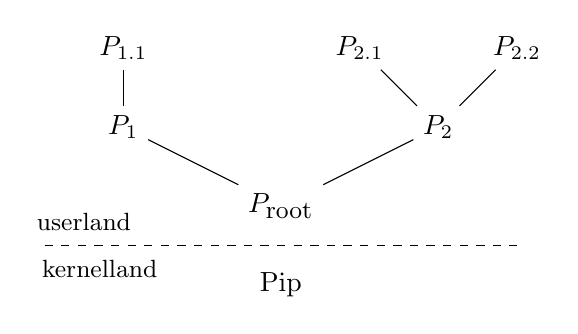
\begin{tikzpicture}
    \node (user) at (-2.5, -0.2) {\small userland};
    \node (kernel) at (-2.3, -0.8) {\small kernelland};
    \node (pip) at (0,-1) {Pip};
    \node (root) at (0,0) {$P_{\mbox{\small root}}$};
    \node (un) at (-2, 1) {$P_1$};
    \node (deux) at (2, 1) {$P_2$};
    \node (unun) at (-2, 2) {$P_{1.1}$};
    \node (deuxun) at (1, 2) {$P_{2.1}$};
    \node (deuxdeux) at (3, 2) {$P_{2.2}$};
    
    %%%%%%%%%%%%%%%%%%%%%%%%%%%%%%%%%%%%%%%%
    
    \draw (root) -- (un);
    \draw (root) -- (deux);
    \draw (un) -- (unun);
    \draw (deux) -- (deuxun);
    \draw (deux) -- (deuxdeux);
    
    \draw[dashed] (-3,-0.5) -- (3,-0.5);
    
\end{tikzpicture}

		\caption{Exemple d'arbre de partition dans Pip}
		\label{fig:partition_tree}
	}
	\end{figure}

	

	\paragraph{Propriété d'isolation} La propriété d'isolation de Pip est divisée en trois sous-propriétés :
	\begin{itemize}
		\item La première, la propriété de \textbf{partage vertical}, stipule que la mémoire partagée par une partition parent avec ses enfants reste accessible au parent par conception.

		\item La seconde, la propriété d'\textbf{isolation horizontale}. Dans Pip, chaque partition peut créer plusieurs partitions enfant ; cependant les portions de mémoire partagées avec chacune doivent être strictement disjointe. Autrement dit, une partition ne peut pas partager une même portion de mémoire avec deux partitions enfant simultanément. Ainsi, deux partitions enfant issues d'une même partition parent sont \emph{isolées} : la mémoire accessible dans l'une d'entre elle est nécessairement inaccessible dans l'autre.

		\item La dernière, la propriété d'\textbf{isolation noyau}. À chaque création de partition, Pip réserve une petite portion de mémoire afin d'y stocker les structures nécessaires au contrôle des droits. Ces portions de mémoire deviennent inaccessibles à n'importe quelle partition.
	\end{itemize}


	\paragraph{Méthodologie de preuve} Pip a pris le contrepied des projets majeurs du domaine en utilisant un \emph{shallow embedding} de C plutôt que d'utiliser un \emph{deep embedding}. Ce \emph{shallow embedding} nécessite l'utilisation d'une monade d'état en Coq (voir \ref{monad}) et d'un outil spécifique (voir $\partial x$ \ref{compilation}) pour reconstruire l'AST ou le code source du noyau pour le compiler.
	Le pari de cette méthodologie est de pouvoir se concentrer sur la sémantique des programmes à prouver afin d'alléger l'effort de preuve général par rapport aux méthodologies utilisant un \emph{deep embedding}. Par ailleurs les proriétés de préservation de l'isolation de Pip ont été prouvées directement plutôt que par raffinement.

	\section{Conclusion}

	\textcolor{red}{Montrer comment ces notions sont reliées par les travaux présentés par la suite}
